\documentclass[a4paper, 10pt]{article}
\usepackage{comment} % enables the use of multi-line comments (\ifx \fi) 
\usepackage{lipsum} %This package just generates Lorem Ipsum filler text. 
\usepackage{fullpage} % changes the margin
\usepackage{epsfig}
\usepackage{listings}

\begin{document}
%Header-Make sure you update this information!!!!
\noindent
\large\textbf{Lab Report:1} \hfill \textbf{Abhishek Srivastava \& Ravdeep Pasricha} \\
\normalsize CS202 Advanced Operating Systems\hfill Student Id: 861307778 \& 861307836 \\
Prof. Nael B. Abu-Ghazaleh \hfill \today \\
\hrule

\noindent
\\
\large\textbf{Problem 1}\\
New system call \textbf{info}\\
\begin{itemize}
\item Files Modified
\begin{itemize}
\item \textbf{defs.h}: Modified for adding system call  \emph{void info(int);}.
	\item \textbf{proc.c}:  Added the definition of \emph{void
	info(int param)} to count the number of process running, number of system call mades and number of memory pages that current process is using.
	\item \textbf{proc.h}: Modified \emph{proc} data structure to add $syscall\_count$ variable to count the number of system calls made by the process.
	\item \textbf{syscall.h}, \textbf{syscall.c}, \textbf{sysproc.c}, \textbf{usys.S}, \textbf{user.h}: Modified to add System call.
	\item \textbf{Makefile}
\end{itemize}
\item File added 
\begin{itemize}
\item \textbf{info.c}
\end{itemize}
\item Functions and System calls added\\
\textbf{Function Added in proc.c}


\begin{lstlisting}
//cs202
void
info(int param)
{ 
  // Process count
  int proc_count = 0;
  // Memory page count
  int pg_count = 0;
  struct proc *p;
  // Travesre the process table and count the process 
  // which are not in unused state.
  for(p=ptable.proc;p<&ptable.proc[NPROC];p++){
    if(p->state != UNUSED){
      proc_count++;
     // cprintf("pid: %d, Name:%s, count: %d \n", p->pid, p->name,
      p->syscall_count);
    }
  }

  // points to the start of the page table
  pde_t *val = proc->pgdir; 
  pde_t *end = (val + proc->sz);
  while (val<end){
    if(*val){
      pg_count++;
      //cprintf("val= %d\n", *val);
    }
    val = val + 4;
  }
  switch(param){
    case 1:
         cprintf("\n Process Count: %d \n", proc_count);
         break;
    case 2:
         // Adding one because counting the "exit" system call
         cprintf("\n Syscall count: %d \n", proc->syscall_count + 1);
         break;
    case 3:
         cprintf("\nPage count: %d\n", pg_count); 
         break;
    default:
         cprintf("\n Wrong Option \n");
         break;
  }  
}
\end{lstlisting}

\textbf{Function added in sysproc.c}
\begin{lstlisting}
//cs202
int
sys_info(void)
{
  int param;
  if(argint(0, &param) < 0){
    return -1;
  }
  info(param);
  return 0;
}
\end{lstlisting}

\textbf{Function added in info.c}
\begin{lstlisting}
#include "types.h"
#include "stat.h"
#include "user.h"


int main(int argc, char *argv[])
{
    info(atoi(argv[1]));
    exit();
}
\end{lstlisting}
\item Result
\begin{figure}
	\centering
	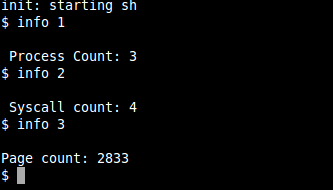
\epsfig{file=part1.png, height=3in, width=6in}
	\caption{info system call output.}
\end{figure}

\end{itemize}

\newpage

\noindent
\large\textbf{Problem 2}\\
Lottery \& Stride Scheduler.\\
 
\noindent
\large\textbf{Solution:}\\
Files Modified:
\begin{itemize}
	\item \textbf{defs.h}: Modified for adding system call  \emph{int sticket(int)}.
	\item \textbf{proc.c}:  Added the definition of \emph{int sticket(int)} to assign the ticket value to the process , increase the count of total tickets, assign the stride value and total stride value for a process, and also modified the round robin scheduler by adding Lottery Scheduler and Stride Scheduler. 
	\item \textbf{proc.h}: Modified \emph{proc} data structure to add 4 more parameters \emph{int tcount,	int tickcount, int stride,	int tstride} for lottery and stride scheduler implementation.
	\item \textbf{syscall.h}, \textbf{syscall.c}, \textbf{sysproc.c}, \textbf{usys.S}, \textbf{user.h}: Modified to add System cal to set ticket, stride value for process.
	\item \textbf{Makefile}:  Added test files \emph{prog1.c, prog2.c, prog3.c, lprog1.c, lprog2.c and lprog3.c}.\\
\end{itemize}
We have recorded the ticks value in the proc data structure. The more the number of tickets the process has the sooner it will finish and lower the number of ticks it will have. \textbf{We have calculated the ratio by summing up the whole number of ticks and dividing the total number of ticks with the number of ticks it took to complete the process}.\\

Results:
Table 1 and Table 2 shows the results of the programs run with ticket values, stride values, number of ticks it took to complete the process and calculated ratio. Figure 2 and Figure 3 shows the screen shots of the results. \\
\newpage
\begin{table}
	\centering
	\caption{Output of Lottery Schedule and calculated ratio}
	\begin{tabular}{|c|c|c|l|} \hline
		Program Name&Ticket Value&Ticks Observer&Calculated Ratio\\ \hline
		lProg1&30&2&5\\ \hline
		lProg2&20&3&3.3\\ \hline
		lProg3&10&10&1\\ \hline
	\end{tabular}
\end{table}
\begin{table}
	\centering
	\caption{Output of Stride Schedule and calculated ratio}
	\begin{tabular}{|c|c|c|c|l|} \hline
		Program Name&Ticket Value&Stride Value&Ticks Observer&Calculated Ratio\\ \hline
		Prog1&100&100&10&1.2\\ \hline
		Prog2&50&250&12&1\\ \hline
		Prog3&250&40&5&2.4\\ \hline
	\end{tabular}
\end{table}
\begin{figure}
	\centering
	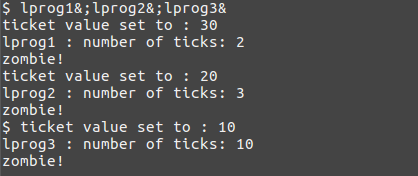
\epsfig{file=OS_SS1_L.png, height=3in, width=6in}
	\caption{Lottery Schedule Output.}
\end{figure}

\begin{figure}
	\centering
	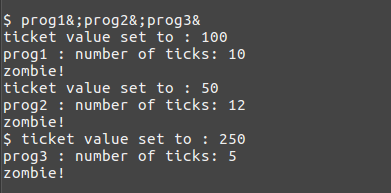
\epsfig{file=OS_SS1_S.png, height=3in, width=6in}
	\caption{Stride Schedule Output.}
\end{figure}
Code Added:

\begin{lstlisting}

/*------------------------------------------------------------------*/

//CS202: System call to set values for the process.
int sticket(int tnum)
{
    //Set the number of tickets to value passed
    proc->tcount = tnum;
    //counter for total number of tickets
    totticket += tnum;
    //calculate the stride value for process
    proc->stride = totstride/tnum;
    proc->tstride = totstride/tnum;
    //For debug purposes
    //cprintf(``ticket value set to : %d\n'', proc->tcount);
    //cprintf(``stride value set to : %d\n'', proc->stride);
}

/*------------------------------------------------------------------*/

// Per-process state
struct proc {
    uint sz;                 // Size of process memory (bytes)
    pde_t* pgdir;            // Page table
    char *kstack;            // Bottom of kernel stack for this process
    enum procstate state;    // Process state
    int pid;                 // Process ID
    struct proc *parent;     // Parent process
    struct trapframe *tf;    // Trap frame for current syscall
    struct context *context; // swtch() here to run process
    void *chan;              // If non-zero, sleeping on chan
    int killed;              // If non-zero, have been killed
    struct file *ofile[NOFILE];  // Open files
    struct inode *cwd;       // Current directory
    char name[16];           // Process name (debugging)
    int tcount;              // CS202 : Ticket Count
    int stride;              // CS202 : Stride value
    int tstride;             // CS202 : Total stride value
    int tickcount;           // CS202 : Ticks calculate
};

/*------------------------------------------------------------------*/

//CS202: Stride Scheduler Implementation
void stride_scheduler(void)
{
    struct proc *p;

    for(;;){
        // Enable interrupts on this processor.
        sti();

        //CS202: Min stride value holder, highest initial value
        int min_stride = totstride;
        //CS202: To store the pid of process with minimum stride value
        int stride_pid = 0;

        // Loop over process table looking for process to run.
        acquire(&ptable.lock);

        //CS202: Loop over the process to find out process with
        //minimum stride value
        for(p = ptable.proc; p < &ptable.proc[NPROC]; p++){
        if(p->state != RUNNABLE)
            continue;

        //CS202: Check if process has the less stride value
        if(p->tstride < min_stride)
        {
            min_stride = p->tstride;
            //store pid value
            stride_pid = p->pid;
        }
    }
    //CS202: Choose the process with pid of minimum stride value
    for(p = ptable.proc; p < &ptable.proc[NPROC]; p++){
        if(p->state != RUNNABLE)
            continue;

        //CS202: Check if process has the pid off minimum stride
        value
        if(p->pid != stride_pid)
            continue;

        // Switch to chosen process.  It is the process's job
        // to release ptable.lock and then reacquire it
        // before jumping back to us.

        //CS202: Increasing the total stride value
        p->tstride += p->stride; 
        proc = p;
        switchuvm(p);
        p->state = RUNNING;
        swtch(&cpu->stride_scheduler, p->context);
        switchkvm();

        //Process is done running for now.
        //It should have changed its p->state before coming back.
        proc = 0;
        }
        release(&ptable.lock);
    }
}

/*------------------------------------------------------------------*/

//CS202: Lottery Scheduler Implementation
void lottery_scheduler(void)
{
    struct proc *p;

    for(;;){
        // Enable interrupts on this processor.
        sti();

        //CS202: Generate random ticket
        int winner = rand()%(totticket+1)
        //CS202: To hold total number of tickets traverssed
        int ticketsum = 0;

        // Loop over process table looking for process to run.
        acquire(&ptable.lock);
        for(p = ptable.proc; p < &ptable.proc[NPROC]; p++){
            if(p->state != RUNNABLE)
                continue;

            //CS202: Condition to choose the process which are runnable
            ticketsum += p->tcount;
            if(ticketsum < winner)
                continue;

            // Switch to chosen process.  It is the process's job
            // to release ptable.lock and then reacquire it
            // before jumping back to us.

            //Increase the count of scheduled number
            proc = p;
            switchuvm(p);
            p->state = RUNNING;
            swtch(&cpu->lottery_scheduler, p->context);
            switchkvm();

            // Process is done running for now.
            // It should have changed its p->state before coming back.
            proc = 0;
        }
        release(&ptable.lock);
    }
}

/*------------------------------------------------------------------*/

//Process Allocation
static struct proc* allocproc(void)
{
    struct proc *p;
    char *sp;

    acquire(&ptable.lock);

    for(p = ptable.proc; p < &ptable.proc[NPROC]; p++)
        if(p->state == UNUSED)
            goto found;

    release(&ptable.lock);
    return 0;

found:
    p->state = EMBRYO;
    p->pid = nextpid++;
    release(&ptable.lock);
  
    // Allocate kernel stack.
    if((p->kstack = kalloc()) == 0){
        p->state = UNUSED;
        return 0;
    }
    sp = p->kstack + KSTACKSIZE;
  
    // Leave room for trap frame.
    sp -= sizeof *p->tf;
    p->tf = (struct trapframe*)sp;
  
    // Set up new context to start executing at forkret,
    // which returns to trapret.
    sp -= 4;
    *(uint*)sp = (uint)trapret;

    sp -= sizeof *p->context;
    p->context = (struct context*)sp;
    memset(p->context, 0, sizeof *p->context);
    p->context->eip = (uint)forkret;

    //CS202: Intialize required ticket values
    p->tcount = 1;
    p->stride = 10;
    p->tstride = 10;
    acquire(&tickslock);
    p->tickcount = ticks;
    release(&tickslock);
    return p;
}

/*------------------------------------------------------------------*/

//CS202: Exit System Call
void exit(void)
{
    struct proc *p;
    int fd;
    //CS202: Final tick value
    acquire(&tickslock);
    if(strlen(proc->name)!=2)
    { 
        cprintf("%s : number of ticks: %d\n",proc->name,
        ticks-proc->tickcount);
    }
    release(&tickslock);
    
    if(proc == initproc)
        panic("init exiting");

    // Close all open files.
    for(fd = 0; fd < NOFILE; fd++){
        if(proc->ofile[fd]){
            fileclose(proc->ofile[fd]);
            proc->ofile[fd] = 0;
        }
    }

    begin_op();
    iput(proc->cwd);
    end_op();
    proc->cwd = 0;

    acquire(&ptable.lock);
    // Parent might be sleeping in wait().
    wakeup1(proc->parent);

    // Pass abandoned children to init.
    for(p = ptable.proc; p < &ptable.proc[NPROC]; p++){
        if(p->parent == proc){
            p->parent = initproc;
            if(p->state == ZOMBIE)
                wakeup1(initproc);
        }
    }
    // Jump into the scheduler, never to return.
    proc->state = ZOMBIE;
    sched();
    panic("zombie exit");
}

/*------------------------------------------------------------------*/

//CS202: simple pseudo-random number generator
//Source: Wikipedia

ushort lfsr = 0xACE1u;
uint bit;

uint rand()
{
    bit  = ((lfsr >> 0)^(lfsr >> 2)^(lfsr >> 3)^(lfsr >> 5))&1;
    return lfsr =  (lfsr >> 1) | (bit << 15);
}


/*------------------------------------------------------------------*/

\end{lstlisting}
\end{document}
